% chktex-file 13

\documentclass[../main]{subfiles}

\begin{document}

\subsection{AREPO}\label{sec:arepo}
Arepo is a massively parallel astrophysics code for the simulation of gravitational N-body systems and magnetohydrodynamics, both on Newtonian as well as cosmological backgrounds.
There are a number of versions in the community, originating from a common closed-source code base.
A version with reduced functionality was made publicly available under GPLv3\cite{weinberger_arepo_2020, springel_arepo_nodate}.
Different research groups use code bases derived from the closed source version, including the Sijaki group at the University of Cambridge.
This code~\cite{sijaki_arepo_nodate}, which was part of the DiRAC3 procurement, acceptance testing and technical commissioning, forms the basis of porting efforts to be undertaken within the course of this project.

In Arepo, the computational domain is discretized using a fully adaptive, dynamic unstructured Voronoi mesh, which is moving with the fluid in a quasi-Lagrangian way and that is paired with a finite volume approach for the hydrodynamics.
Arepo is written in C, parallelized with MPI and some of the code bases, including the one used in this project, have additionally OpenMP shared memory parallelization.
To the best of our knowledge, there is currently no version of this code that can target accelerators with any of the computational kernels in the main time loop.

\subsubsection{Running the code}
Arepo depends on several libraries that are necessary for compilation. 
    \begin{itemize}
        \item{\textbf{GSL\footnote{\url{https://www.gnu.org/software/gsl}}:}} GNU Scientific Library as a random number generator and for numerical integration.
        \item{\textbf{GMP \footnote{\url{https://gmplib.org/}}:}} GNU Multiple Precision Artithmetic Library to calculate exact geometric predictions
        \item{\textbf{FFTW3\footnote{\url{http://www.fftw.org/}}:}} Fastest Fourier Transform in the West is used in the particle-mesh algorithm
        \item{\textbf{HDF5\footnote{\url{https://support.hdfgroup.org/HDF5/doc/H5.intro.html}}:}} Hierarchical Data Format is used as the standard input/output format in Arepo. 
    \end{itemize}
Additionally Arepo needs a configuration and a parameter file for each example. The parameter File contains the run-time options whereas the configuration file specifies the code and is needed at compile-time. Special variables in the parameter file needs to be modified on each platform to provide the maximum memory size, which should be around 95\% of the available RAM for every process and it must point to the correct data folder for initial condition files and output files. Most Arepo branches come with a testsuite of small examples to verify the code. Furthermore Arepo was used in the Illustris project\footnote{\url{https://www.illustris-project.org/}} and test data from that project~\cite{Nelson_2015} can be used for longer test runs. The Illustris examples require a path to an empty file named 'ExpansionList\_128'. 

\subsubsection{Profiling with Vtune}
In contrast to codes described above, where suitable kernels for GPU execution have already been identified in prior porting efforts, this selection process has to be done as an additional first step for this purely CPU-based code.
Therefore, extensive profiling of the code base has been undertaken using one of the test cases that are also used to verify code correctness to analyze the potential of porting parts of Arepo to GPUs.
Hence, a first analysis was carried out using Intel VTune profiler and Intel Trace Analyzer, producing two key insights:

The first insight was that a significant share of the overall run time is spent waiting in a synchronisation step that uses global MPI communication.
The purpose of this step is to detect the need for program interruption to trigger saving the current state in a snapshot file and termination of the program.
Since there is no data dependence on this communication step, it is possible to reverse the logic of this routine, replace the respective MPI calls with their non-blocking counterparts and trigger the snapshot writing after the next time step.
This enables perfect overlap of computation and communication at the expense of a one time step lag in the snapshot writing.
Figure \ref{fig:arepo_mpicom} shows the comparison of the blocking (top) vs the nonblocking (bottom) synchronisation step for a random selection of MPI tasks. It is clearly visible that the MPI busy wait portion of the code (yellow), i. e.  the time that a rank is waiting for others to reach the synchronisation point, is reduced in the graphical output where nonblocking communication is used. 

\begin{figure}[htp]
	\centering
	\subfloat{ 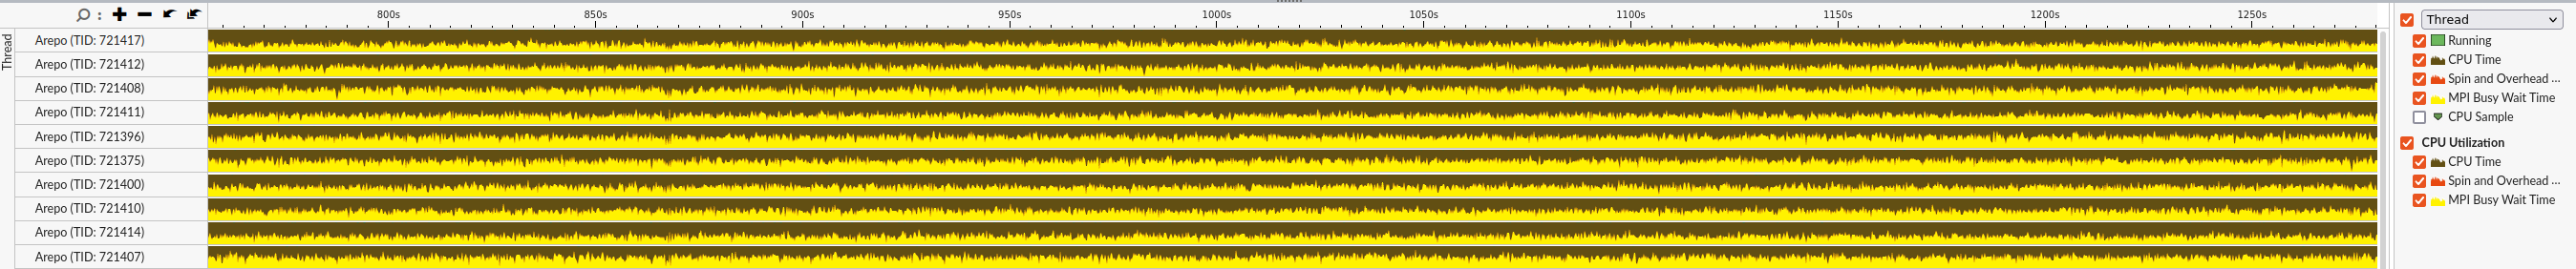
\includegraphics[clip,width=\textwidth]{arepo_blocking.png}}\\
	\subfloat{ 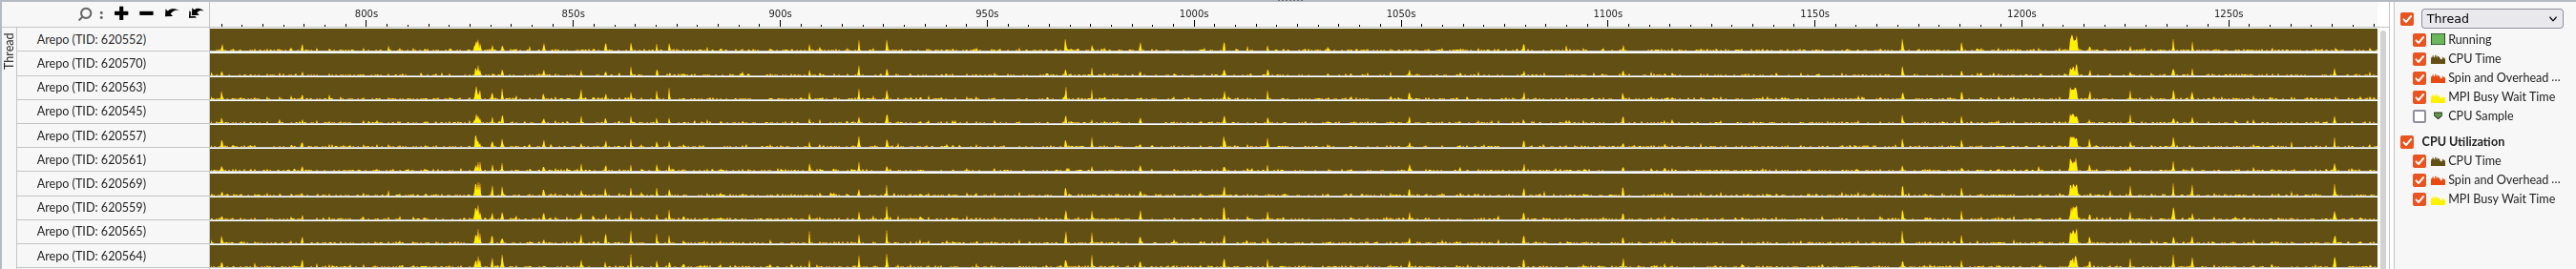
\includegraphics[clip,width=\textwidth]{arepo_nonblocking.png}}
	\caption{Significant reduction of MPI Busy Wait Time (yellow) in the lower VTune Profiler graphic compared to the top version where blocking communication was used. Shown for a random selection of ranks}
	\label{fig:arepo_mpicom} % chktex 24
\end{figure}
To further test these findings, the Illustris 3 testcase [2] was used. Figure \ref{fig:arepo_blockvsnonblock} shows the impact of this improvement across varying number of MPI tasks by comparing overall runtime of the original code variant (blue line) with the improved version (orange line). As expected, the synchronisation overhead is negligible for smaller numbers of tasks where computational work dominates but becomes noticeable with more than ~2000 tasks and incurs significant slow-down with ~3000 tasks and more.  
\begin{figure}[htp]
	\centering
	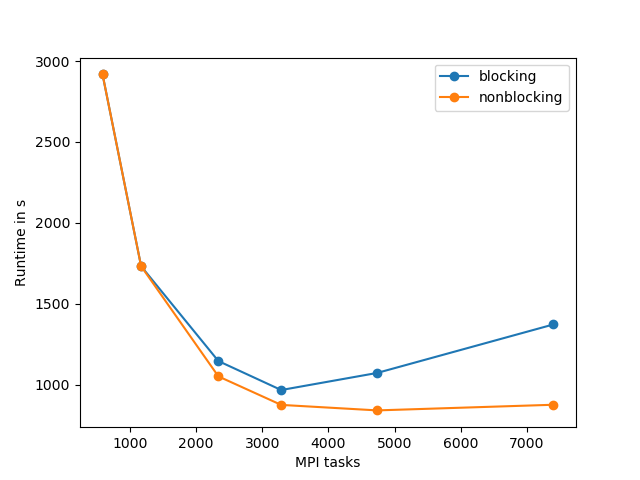
\includegraphics[clip,width=0.6\textwidth]{images/Arepo_blockingvsNonblocking.png}
	\caption{A comparison between the blocking and nonblocking synchronization step for }
	\label{fig:arepo_blockvsnonblock} % chktex 24
\end{figure}
Second profiling outcome and original motivation for this analysis was to understand the distribution of run time across the different parts of a time step and subsequently to identify suitable candidates for GPU porting.
The two most time-consuming parts proved to be the evaluation of gravitational forces, which is carried out in two half steps at the beginning and end of a time step, and the creation of the Voronoi mesh in-between.

 \subsubsection{OneAPI Offload Advisor}
The next step in the analysis was to use Intel's Offload Advisor to see if these contain any kernels that would readily benefit from GPU offloading.
However, with the current structure of the underlying algorithm the Offload Advisor judged every routine to suffer from too much overhead when ported to GPU.
Only relatively short loops within sub steps of the mesh creation routines were classified as offload candidates that could potentially see any speed-up.

Overall, this suggests that for a successful GPU port of Arepo it may not be sufficient to port few individual kernels to achieve performance gains but requires a better understanding of the numerical method and possibly adaptation of the algorithm to better map to the target hardware.
For that, we are in active discussions with the developers at the University of Cambridge and take into account prior experience and publications in the scientific domain.

\subsubsection{Intel oneAPI Math Kernel Library}



%As a C application that includes already OpenMP parallelization, we intend to follow Intel's recommendation to use OpenMP 5 offloading to target GPUs.


%\begin{itemize}
%    \item reference to paper to port
%    \item https://arxiv.org/abs/1610.07279
%    \item https://arxiv.org/abs/0907.3390
%    \item https://arxiv.org/abs/1909.07439
%\end{itemize}

\end{document}
